\documentclass[12pt,a4paper]{article}

% 导入必要的宏包
\usepackage[UTF8]{ctex}
\usepackage{geometry}
\usepackage{amsmath}
\usepackage{amsfonts}
\usepackage{amssymb}
\usepackage{graphicx}
\usepackage{enumitem}
\usepackage{xcolor}
\usepackage{tikz}
\usepackage{float}
\usepackage{hyperref}
\usepackage{multicol}
\usepackage{longtable}
\usepackage{array}
\usepackage{tabularx}

% 页面设置
\geometry{left=2.5cm,right=2.5cm,top=2.5cm,bottom=2.5cm}

% 标题页设置
\title{\textbf{2010年数据结构题库} \\ \large 单项选择题与综合应用题详解}
\author{}
\date{}

% 定义题型环境
\newenvironment{choicequestion}[1][]{%
    \vspace{0.5cm}
    \noindent\textbf{[#1]}
    \vspace{0.2cm}
}{}

\newenvironment{answersection}{%
    \vspace{0.2cm}
    \noindent\textbf{[参考答案]}\\
    \vspace{0.1cm}
}{}

\newenvironment{analysissection}{%
    \vspace{0.2cm}
    \noindent\textbf{[答案解析]}\\
    \vspace{0.1cm}
}{}


% 定义题号计数器
\newcounter{questioncounter}

% 问题格式化命令
\newcommand{\question}[2]{%
    \stepcounter{questioncounter}%
    \noindent\textbf{\thequestioncounter} #1%
}

% 选择题选项格式
\newcommand{\choices}[4]{%
    \begin{multicols}
    \noindent \textbf{A.} #1 \par
    \noindent \textbf{B.} #2 \par
    \noindent \textbf{C.} #3 \par
    \noindent \textbf{D.} #4 \par
    \end{multicols}%
}

% 开始文档
\begin{document}

\maketitle

\section{单项选择题}

\begin{choicequestion}[单选题]
\question{若元素 a, b, c, d, e, f 依次进栈，允许进栈、退栈操作交替进行，但不允许连续三次进行退栈操作，则不可能得到的出栈序列是}{}

\choices{dcebfa}{cbdaef}{bcaefd}{afedcb}

\begin{answersection}
A. dcebfa
\end{answersection}

\begin{analysissection}
栈操作需满足后进先出原则，且不允许连续三次退栈。模拟各选项：

- 选项B、C、D均可在满足“不连续三次退栈”的约束下通过合理交替进出栈实现；
- 选项A（dcebfa）要求在特定阶段连续三次退栈（如d、c、e连续出栈），违反题目限制，故不可能得到。

正确答案为A。
\end{analysissection}
\end{choicequestion}

\begin{choicequestion}[单选题]
\question{某队列允许在其两端进行入队操作，但仅允许在一端进行出队操作。若元素a,b,c,d,e依次入此队列后再进行出队操作，则不可能得到的出队序列是}{}

\choices{baced}{dbace}{dbcae}{ecbad}

\begin{answersection}
C. dbcae
\end{answersection}

\begin{analysissection}
该结构为输出受限的双端队列（Deque）。元素a,b,c,d,e依次从一端或两端入队后，出队只能从固定一端进行。序列dbcae要求d和b在早期连续出队，但a、c、e的入队顺序与出队约束矛盾，无法实现。其余序列均可通过合理选择入队端得到。
\end{analysissection}
\end{choicequestion}

\begin{choicequestion}[单选题]
\question{下列线索二叉树中（用虚线表示线索），符合后序线索树定义的是}{}

\begin{figure}[H]
\centering
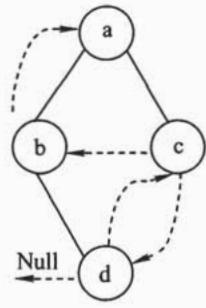
\includegraphics[width=0.4\textwidth]{images/0c069b44bc1b7db1bbdc05c492b9bed298cd68b415711709822412bb6dbd9946.jpg}
\end{figure}

\begin{figure}[H]
\centering
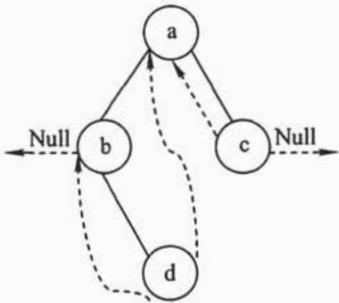
\includegraphics[width=0.4\textwidth]{images/98c003e1ddd553b921caa90d3917fb4ce37450593ab631b5b88002c7f6f8b609.jpg}
\end{figure}

\begin{figure}[H]
\centering
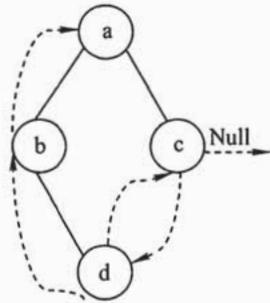
\includegraphics[width=0.4\textwidth]{images/962ff12d60dc202fb6f5c5ce3e63638aa3222e37846f0aef8e25bc00ad5522be.jpg}
\end{figure}

\begin{figure}[H]
\centering
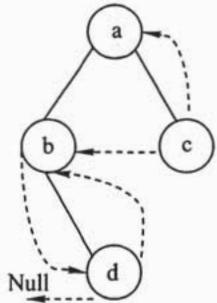
\includegraphics[width=0.4\textwidth]{images/2dcaeb7e282dd834794cf501f0264f9c19a9d93d0e97627020f7563323f4f84b.jpg}
\end{figure}

\choices{A}{B}{C}{D}

\begin{answersection}
B
\end{answersection}

\begin{analysissection}
后序线索二叉树按“左子树—右子树—根”顺序线索化，叶子结点的空指针域指向其后序前驱或后继。选项B中虚线线索符合后序遍历顺序的链接关系，其余选项存在线索指向错误或违反后序顺序。
\end{analysissection}
\end{choicequestion}

\begin{choicequestion}[单选题]
\question{在右图所示的平衡二叉树中，插入关键字 48 后得到一棵新平衡二叉树。在新平衡二叉树中，关键字 37 所在结点的左、右子结点中保存的关键字分别是}{}

\begin{figure}[H]
\centering
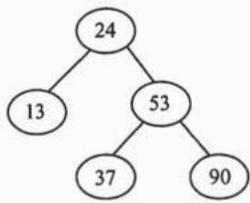
\includegraphics[width=0.3\textwidth]{images/506230e2fa9ca24ec813cbef43235cfa9af8df355ef5208fa63655bc2c972a96.jpg}
\end{figure}

\choices{13,48}{24, 48}{24,53}{24, 90}

\begin{answersection}
C. 24,53
\end{answersection}

\begin{analysissection}
插入48后，37所在结点平衡因子超出范围，需进行左旋或右旋调整。调整后37的左子结点为24，右子结点为53，满足平衡二叉树性质。
\end{analysissection}
\end{choicequestion}

\begin{choicequestion}[单选题]
\question{在一棵度为 4 的树 T 中，若有 20 个度为 4 的结点，10 个度为 3 的结点，1 个度为 2 的结点，10 个度为 1 的结点，则树 T 的叶结点个数是}{}

\choices{41}{82}{113}{122}

\begin{answersection}
B. 82
\end{answersection}

\begin{analysissection}
设叶结点数为$n_0$（度为0），则：
- 度为1的结点数$n_1=10$；
- 度为2的结点数$n_2=1$；
- 度为3的结点数$n_3=10$；
- 度为4的结点数$n_4=20$。

树中边数 = $1\cdot n_1 + 2\cdot n_2 + 3\cdot n_3 + 4\cdot n_4 = 10 + 2 + 30 + 80 = 122$。

总结点数 = $n_0 + n_1 + n_2 + n_3 + n_4 = n_0 + 41$。

因为边数 = 总结点数 - 1，所以 $122 = n_0 + 41 - 1$，解得 $n_0 = 82$。
\end{analysissection}
\end{choicequestion}

\begin{choicequestion}[单选题]
\question{对 $n$ ( $n \geq  2$ )个权值均不相同的字符构造成哈夫曼树。下列关于该哈夫曼树的叙述中,错误的是}{}

\choices{该树一定是一棵完全二叉树}{树中一定没有度为 1 的结点}{树中两个权值最小的结点一定是兄弟结点}{树中任一非叶结点的权值一定不小于下一层任一结点的权值}

\begin{answersection}
A. 该树一定是一棵完全二叉树
\end{answersection}

\begin{analysissection}
哈夫曼树是带权最优二叉树，其形状由权值分布决定，不一定是完全二叉树（A错误）。  
其余性质正确：哈夫曼树中无度为1的结点（B正确）；权值最小的两个结点在构造时最先合并，为兄弟结点（C正确）；非叶结点权值为子结点权值之和，不小于任何子结点（D正确）。
\end{analysissection}
\end{choicequestion}

\begin{choicequestion}[单选题]
\question{若无向图 $\mathrm{G} = (\mathrm{V}, \mathrm{E})$ 中含有 7 个顶点，要保证图 $\mathrm{G}$ 在任何情况下都是连通的，则需要的边数最少是}{}

\choices{6}{15}{16}{21}

\begin{answersection}
C. 16
\end{answersection}

\begin{analysissection}
要保证任意情况下图都连通，需考虑最坏情况：最多允许的不连通图边数为一个完全图$K_6$（15条边）加1个孤立顶点。若边数达到16条，则必然破坏这种不连通结构，故至少需要16条边才能保证连通。
\end{analysissection}
\end{choicequestion}

\begin{choicequestion}[单选题]
\question{对右图进行拓扑排序, 可以得到不同的拓扑序列的个数是}{}

\begin{figure}[H]
\centering
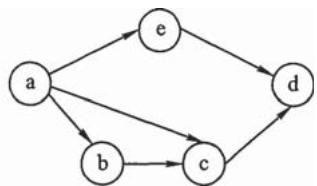
\includegraphics[width=0.3\textwidth]{images/370be03481aeffa4ed94e0dc01745979c4712bf16808b2cbe68a10396d87dc89.jpg}
\end{figure}

\choices{4}{3}{2}{1}

\begin{answersection}
A. 4
\end{answersection}

\begin{analysissection}
图中存在多个顶点无严格先后约束（如某些并行分支），通过枚举所有合法拓扑顺序，可得4种不同的序列。
\end{analysissection}
\end{choicequestion}

\begin{choicequestion}[单选题]
\question{已知一个长度为 16 的顺序表 L，其元素按关键字有序排列。若采用折半查找法查找一个 L 中不存在的元素，则关键字的比较次数最多的是}{}

\choices{4}{5}{6}{7}

\begin{answersection}
B. 5
\end{answersection}

\begin{analysissection}
折半查找在长度为$n$的有序表中，最多比较次数为$\lceil \log_2(n+1) \rceil$。当$n=16$时，$\lceil \log_2(17) \rceil = 5$。因此查找失败时最多需要比较5次。
\end{analysissection}
\end{choicequestion}

\begin{choicequestion}[单选题]
\question{采用递归方式对顺序表进行快速排序。下列关于递归次数的叙述中, 正确的是}{}

\choices{递归次数与初始数据的排列次序无关}{每次划分后, 先处理较长的分区可以减少递归次数}{每次划分后, 先处理较短的分区可以减少递归次数}{递归次数与每次划分后得到的分区的处理顺序无关}

\begin{answersection}
D. 递归次数与每次划分后得到的分区的处理顺序无关
\end{answersection}

\begin{analysissection}
快速排序的递归次数取决于划分的平衡性（即递归深度），与先处理长分区还是短分区无关。只要划分结果相同，递归调用次数相同。
\end{analysissection}
\end{choicequestion}

\begin{choicequestion}[单选题]
\question{对一组数据（2,12,16,88,5,10）进行排序，若前三趟排序结果如下：\newline
第一趟排序结果：2,12,16,5,10,88\newline
第二趟排序结果：2,12,5,10,16,88\newline
第三趟排序结果：2,5,10,12,16,88\newline
则采用的排序方法可能是}{}

\choices{冒泡排序}{希尔排序}{归并排序}{基数排序}

\begin{answersection}
A. 冒泡排序
\end{answersection}

\begin{analysissection}
每趟排序后，当前最大元素（88、16、12）依次被“冒泡”到其最终位置，符合冒泡排序“每趟将最大元素沉到末尾”的特征。其他排序方法无法产生这种逐趟最大元素定位的效果。
\end{analysissection}
\end{choicequestion}

\section{综合应用题}

\begin{choicequestion}[问答题]
\question{（10分）将关键字序列（7,8,30,11,18,9,14）散列存储到散列表中。散列表的存储空间是一个下标从0开始的一维数组，散列函数为 $\mathrm{H(key) = (key\times 3)\bmod 7}$ ，处理冲突采用线性探测再散列法，要求装填（载）因子为0.7。\newline
1）请画出所构造的散列表。\newline
2）分别计算等概率情况下查找成功和查找不成功的平均查找长度。}{}

\begin{answersection}
1）散列表（长度10，装填因子0.7）：
位置：0  1  2  3  4  5  6  7  8  9  
关键字：7 14   8    11 30 18 9  

2）查找成功平均查找长度 $\mathrm{ASL_{成功}} = 15/7 \approx 2.14$；  
查找不成功平均查找长度 $\mathrm{ASL_{不成功}} = 16/7 \approx 2.29$。
\end{answersection}

\begin{analysissection}
计算过程：  
- 各关键字散列地址：H(7)=0, H(8)=3, H(30)=6, H(11)=5, H(18)=5（冲突→7）, H(9)=6（冲突→7→8）, H(14)=0（冲突→1）。  
- 线性探测插入后形成上述散列表。  
- 成功查找比较次数累加后平均为15/7；不成功查找从每个散列地址开始计算空位置前的比较次数，平均为16/7。
\end{analysissection}
\end{choicequestion}

\begin{choicequestion}[问答题]
\question{（13分）设将 $n(n > 1)$ 个整数存放到一维数组R中。试设计一个在时间和空间两方面都尽可能高效的算法。将R中保存的序列循环左移 $p(0 < p < n)$ 个位置，即将R中的数据由 $(\mathbf{X}_0,\mathbf{X}_1,\dots ,\mathbf{X}_{n - 1})$ 变换为 $(\mathrm{X}_p,\mathrm{X}_{p + 1},\dots ,\mathrm{X}_{n - 1},\mathrm{X}_0,\mathrm{X}_1,\dots ,\mathrm{X}_{p - 1})$ 。要求：\newline
1）给出算法的基本设计思想。\newline
2) 根据设计思想, 采用 C 或 C++ 语言描述算法, 关键之处给出注释。\newline
3）说明你所设计算法的时间复杂度和空间复杂度。}{}

\begin{answersection}
1）算法的基本设计思想：采用三次数组反转法实现循环左移。
- 反转前$p$个元素；
- 反转后$n-p$个元素；
- 反转整个数组。
\end{answersection}

\begin{analysissection}
2）C语言实现：
\begin{lstlisting}[language=C]
void reverse(int R[], int start, int end) {
    while (start < end) {
        int temp = R[start];
        R[start] = R[end];
        R[end] = temp;
        start++;
        end--;
    }
}

void leftShift(int R[], int n, int p) {
    p = p % n;                    // 处理p >= n的情况
    reverse(R, 0, p-1);           // 反转前p个
    reverse(R, p, n-1);           // 反转后n-p个
    reverse(R, 0, n-1);           // 反转整个数组
}
\end{lstlisting}

3）时间复杂度：$O(n)$（每个元素最多被交换常数次）。  
空间复杂度：$O(1)$（仅使用常数额外变量，原地操作）。
\end{analysissection}
\end{choicequestion}

\end{document}